\documentclass[11pt,a4paper]{article}
\usepackage[latin1]{inputenc}
\usepackage[top=1in,bottom=1in,left=0.75in,right=0.75in]{geometry}
\usepackage{amsmath}
\usepackage{soul}
\usepackage{hyperref}
\usepackage{listings}
\usepackage{lastpage} % for the number of the last page in the document
\usepackage{fancyhdr}
\pagestyle{fancy}
\usepackage{graphicx}
\usepackage[table]{xcolor}
\usepackage{framed}
\usepackage{tabularx}
\setlength\parindent{0cm}
\setlength{\parskip}{0.15cm}%
\usepackage{longtable}
\usepackage{wrapfig}
\fancyhf{}
\fboxrule=4pt%border thickness
\lhead{Documentation}
\rhead{Project Plan}
\usepackage{graphicx}
\usepackage{subfig}

\lfoot{}
\rfoot{Page \thepage\ of \pageref{LastPage}}\usepackage{amsfonts}
\usepackage{amssymb}

\begin{document}
\pagenumbering{gobble}

\pagenumbering{gobble}
\begin{titlepage}

\newcommand{\HRule}{\rule{\linewidth}{0.5mm}} % Defines a new command for the horizontal lines, change thickness here

\center % Center everything on the page


\includegraphics[scale=0.4]{images/aber.png} \\[1.5cm] % Name of your university/college
\textsc{\Large Aberystwyth University
 \\[0.5cm] Department of Computer Science}

\

\textsc{\Large Project AWESOME}\\

\HRule \\[0.4cm]
{ \huge  Project Plan}\\[0.4cm] % Title of your document
\HRule \\[1.5cm]

\Large \emph{Author:}\\
Keiron \textsc{O'Shea (keo7@aber.ac.uk)}\\[1cm] % Your name 

{\large June 2014}\\[2cm] % Date, change the \today to a set date if you want to be precise

\


\small version: 0.5 \\
\small status: draft


\vfill % Fill the rest of the page with whitespace

\end{titlepage}

\thispagestyle{plain}	

\tableofcontents

\clearpage

\pagenumbering{arabic}

\clearpage

\section{Introduction}

\subsection{Purpose of this document}


The purpose of this document is to present how I've translated the project brief, the Aberystwyth Web Evaluation Surveys Of Module Experiences (AWESOME), a web-based module evaluation questionnaire generator for the monitoring and evaluation of teaching, into subsystems of objectives and milestones.

Moreover this document will describe the various interactions between separate components of the system and outline initial ideas surrounding the visual appearance of the user interface.

This document will also discuss project management with the use of a Gantt Chart, providing an overview of the project's major tasks and related milestones. This will coexist with a probabilistic analysis of risks, of which will cover some main issues that may occur throughout the development of the project.

\subsection{Scope}

The project plan should intend to give an overview of the proposed system, including a brief description of platforms and HLA - as well as provide a description of target users. It will also contain a user case diagram that aims to give an overview of how the users might interact with each-other. An idea of the user-interface design will also be provided with descriptions of how it will interact with the end user. In terms of project management, a Gantt chart will be used to display the start and end dates fo rthe main tasks of the project and a risk analysis that will highlight issues the project may encounter.

\subsection{Objectives}

The objectives of this particular document are:

\begin{itemize}
	\item to describe the appearance of the user interface.
	\item to indicate an understanding of user behaviour.
	\item give further indication of the proposed time-line surrounding the development of the project.
	\item to indicate an understanding of the risks and other factors of the project.
\end{itemize}

\clearpage

\section{Overview}

The "Aberystwyth Web Evaluation Surveys Of Module Experiences", or AWESOME for short, is a web-based module evaluation questionnaire generator for the monitoring and evaluation of teaching.

\subsection{Platforms and High Level Architecture}

I intend to use the following platforms for the system.

\subsubsection{Hypertext Markup Language (HTML)}

The project brief stated specifically that the system is to be deployed completely via the web. We will be using  Hypertext Markup Language (HTML) as the markup language used to create the application.

\subsubsection{Cascading Style Sheets (CSS)}

In order to produce an aesthetically-pleasing web application I will utilise CSS to specify the styles of the visual elements of the website.

\subsubsection{PHP: Hypertext Preprocessor (PHP)}

On the server side PHP will be used to handle communication between the client and the database and handle the creation of the questionnaires as well as providing dynamic web pages. PHP is widely available on the majority (if not all) web servers and is relatively easy to deploy compared to similar systems.

\subsubsection{PostgreSQL}

PostgreSQL is one of the most widely used database platforms and will be used to store application information. The platform is renowned for its simplistic commands and is easily deployed and managed.

\

The high level architecture consists of the following elements and application mechanics;

\subsubsection{Analytics}

For staff to analyse feedback analytics consisting of visually-appealing graphs and textual responses will be rendered.

\subsubsection{Internet Connectivity}

Both staff and students will require connection to the server to allow them to use the application. Google Charts has been pinpointed as a possible way of doing this as it comes with a readily available API, and still keeps in line with the approach of using free software to build the entire system.

\subsubsection{Staff Access to SAMS/AStRA}

In order to retrieve module information both both staff and students we would like to utilise either SAMS (Student Attendance Monitoring System) or AStRA (Aberystwyth Student Records and Admissions). Both of these systems require staff authentication.

\subsubsection{Generate student questionnaires}

We need to ensure that the questions asked are relevant to the module. An example could be that in the Department of Computer Science we could have department-level questions (about certain rooms, or advisory). Although not a necessity, AWESOME needs to be robust and portable enough to extend so that other departments can also ask specific questions.

Most, if not all questionnaires will contain questions such as:

\begin{itemize}
	\item "Rate this on a scale of 1-5"
	\item Multiple 
\end{itemize}

\subsubsection{Collate feedback}

This component is activated when a student submits a completed questionnaire. In order to ensure that the responses are completely anonymous it will store the answers to the database with no record of the user ID of the submitter. Ideally it would be easy to export the data to a format for processing in Microsoft Excel/LibreOffice Calc (CSV)- we also aim to utilise the stored data to implement some visualisation on the AWESOME website.

\subsubsection{Automated targeted reminder emails}

\subsection{Description of Target Users}

All design must begin with the understanding of who the user is, but due to the relatively large range of age and expertise of the target-base this will be difficult to achieve. The proposed system will be targeted to both staff and students who are currently working or studying at a higher education institute. Because of this inability to pinpoint a specific user base, it would be best to ensure that when designing the user interface we need to ensure that the application is simple to use (in order to avoid frustration and confusing) it must also be informative.

\clearpage

\section{Use Case}


\subsection{Use Case Diagram}

\subsection{Use Case Descriptions}
\clearpage
\section{User interface design}

\subsection{User Navigation}

Below is a flow diagram which describe how the application is navigated.

\begin{figure}[h]
\centering
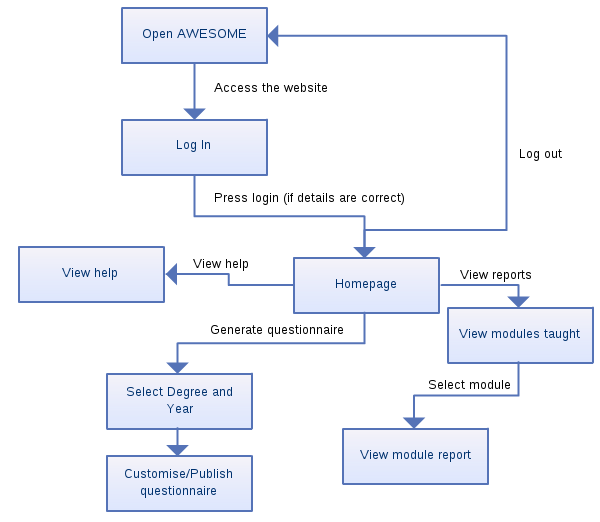
\includegraphics[width=0.85\linewidth]{images/flow/flow.png}
\end{figure}

\clearpage

\subsection{GUI Design}

The following images cover the initial concept of the application. These designs were made using bootstrap and can be accessed at the following url:

\url{http://htmlpreview.github.io/?https://github.com/KeironO/AWESOME/blob/master/Prototyping/UIDesign/index.html}

\subsubsection{Home Page}
The homepage is the first view to be presented to the applications user, inviting them to log onto the AWESOME system by entering their staff credentials for the e-mail address and password fields that are to be validated by the server upon the push of the login button. Inline with other BIS systems, a warning will be placed announcing that you need to be a member of staff of the University to have access to this system.

The page will also consist of a section consisting of news surrounding the AWESOME system. It's important to keep staff informed of expected downtime due to maintenance.
\begin{figure}[h]
\centering
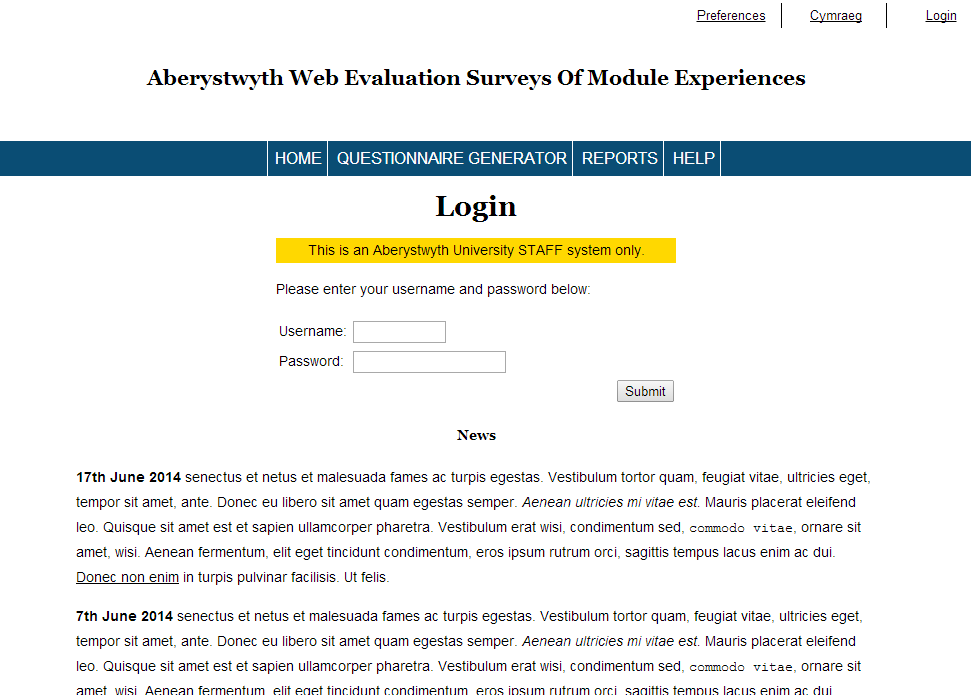
\includegraphics[width=0.85\linewidth]{images/uidesign/homepage.png}
\end{figure}

\clearpage

\subsubsection{Questionnaire Home}

Once the user has successfully logged in using the correct credentials they can then have full access to the AWESOME system. On the homepage of the questionnaire generator the user will be greeted by options of what degree scheme and year they would like to send a questionnaire to. Underneath each year the number of students enrolled for that year will be listed.

\begin{figure}[h]
\centering
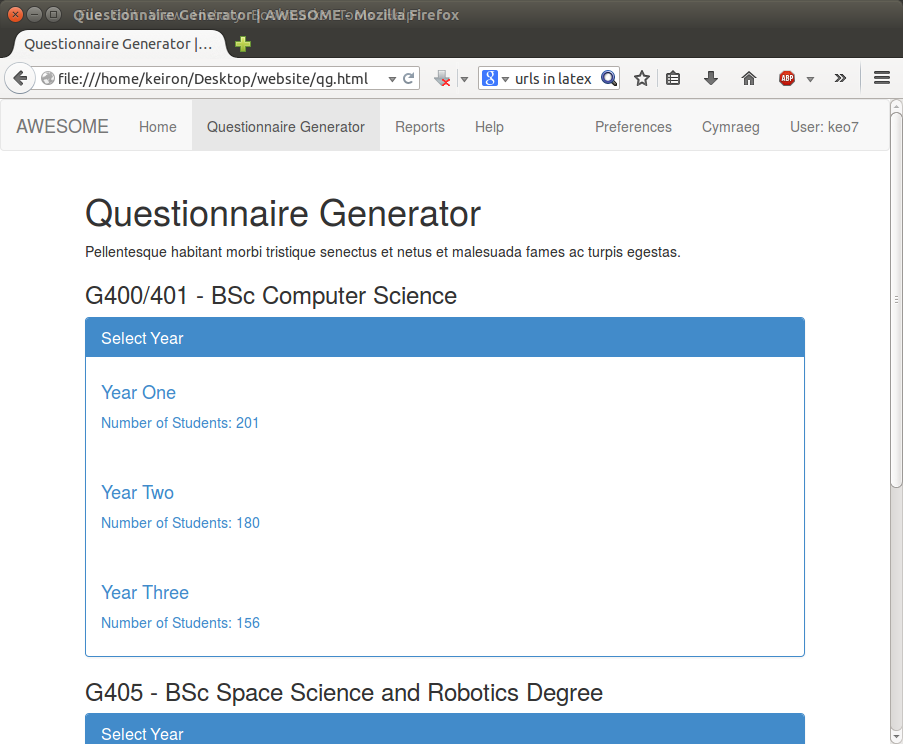
\includegraphics[width=0.85\linewidth]{images/uidesign/questionnairehome.png}
\end{figure}

\clearpage

\subsubsection{Generating a Questionnaire}

Once the user has selected what degree and year they would like to generate a questionnaire for, they will be redirected to the questionnaire generator which will display all modules on offer for that particular degree/year and give the option to add additional (\textit{special/departmental}) questions.

Although not in the figure below, it may be a good idea to also show the members of staff that teach that module as well as the number students enrolled on each module. I also plan on giving a checkbox to allow for 'quick' questionnaires. These will only consist of the "one-question-per-module" schema.

\begin{figure}[h]
\centering
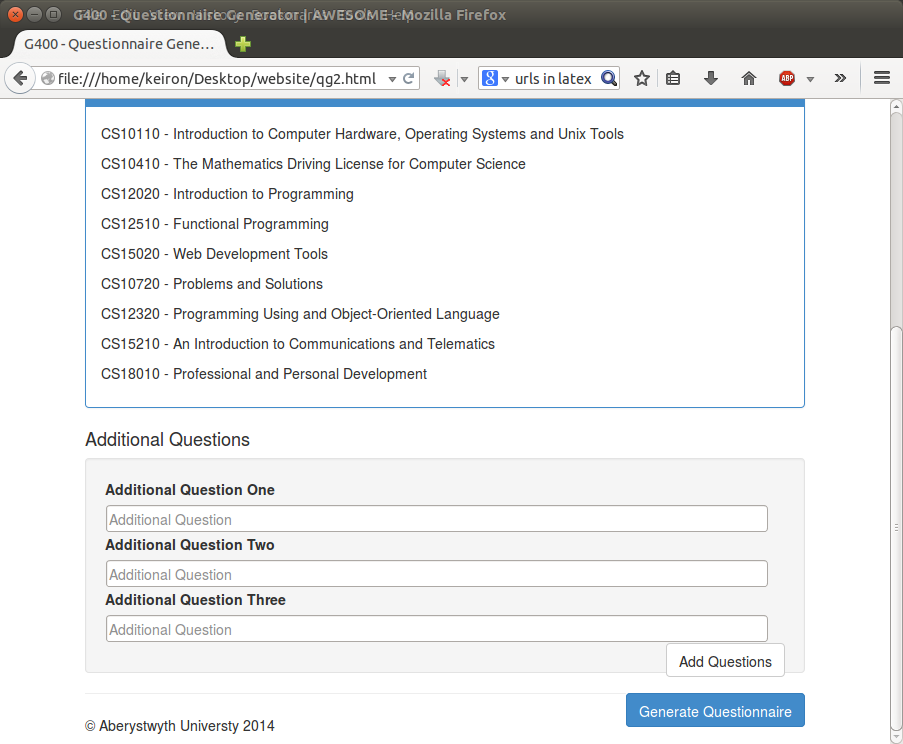
\includegraphics[width=0.85\linewidth]{images/uidesign/generatingquestionnaire.png}
\end{figure}

\clearpage

\subsubsection{Vetting a Questionnaire}

After additional questions have been added and the user has generated a questionnaire, they will then be able view the questionnaire and make any desired changes.

Once finished, a button will be provided in order to email the survey out to the students.

\begin{figure}[h]
\centering
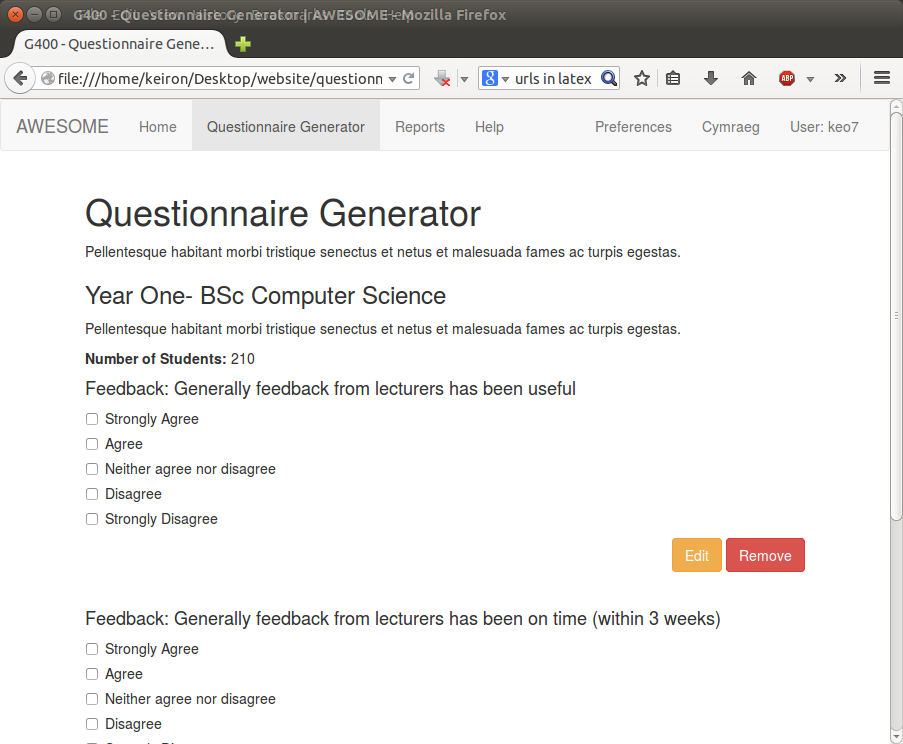
\includegraphics[width=0.85\linewidth]{images/uidesign/vettingquestionnaire.png}
\end{figure}

\clearpage

\subsubsection{Student Questionnaire}

This will be the webpage sent out to the students, it will contain simple instructions as well as a progress bar to ensure that the student knows how long until they have successfully completed the questionnaire.

Once they have completed the questionnaire, a dialogue box will appear congratulating the user upon his/hers completion.

\begin{figure}[h]
\centering
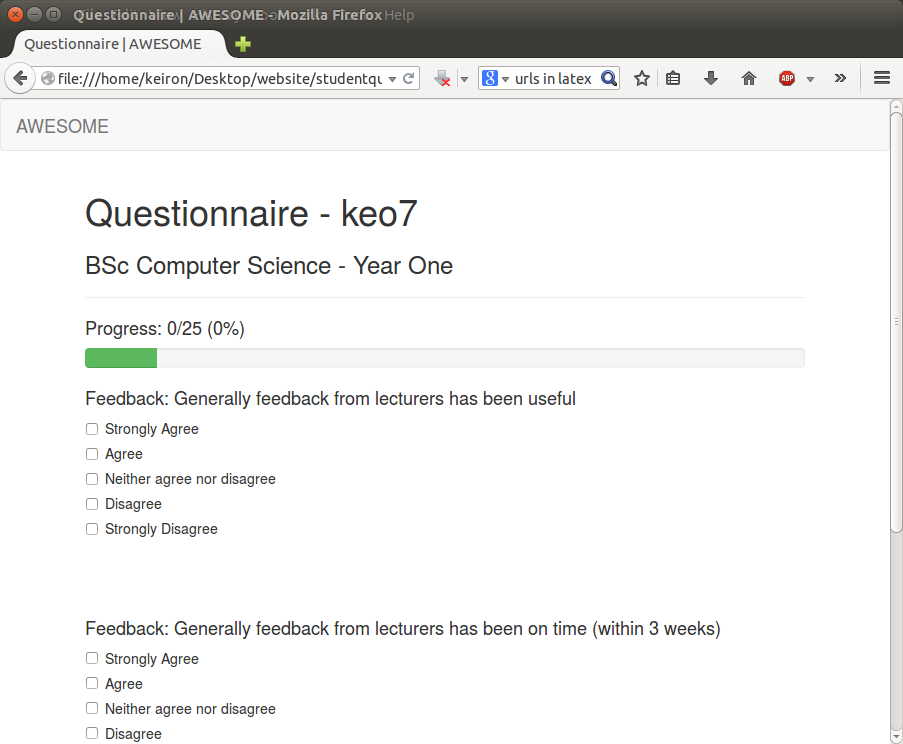
\includegraphics[width=0.85\linewidth]{images/uidesign/studentquestionnaire.png}
\end{figure}

\clearpage

\subsubsection{Reports Home}

The reports page will consist of all the feedback available for that member of staff to look at, consisting of both modules taught and their department. It may also be a good idea to allow the comparison of departmental performance, but this does not feature in the prototype.

\begin{figure}[hbtp]
\centering
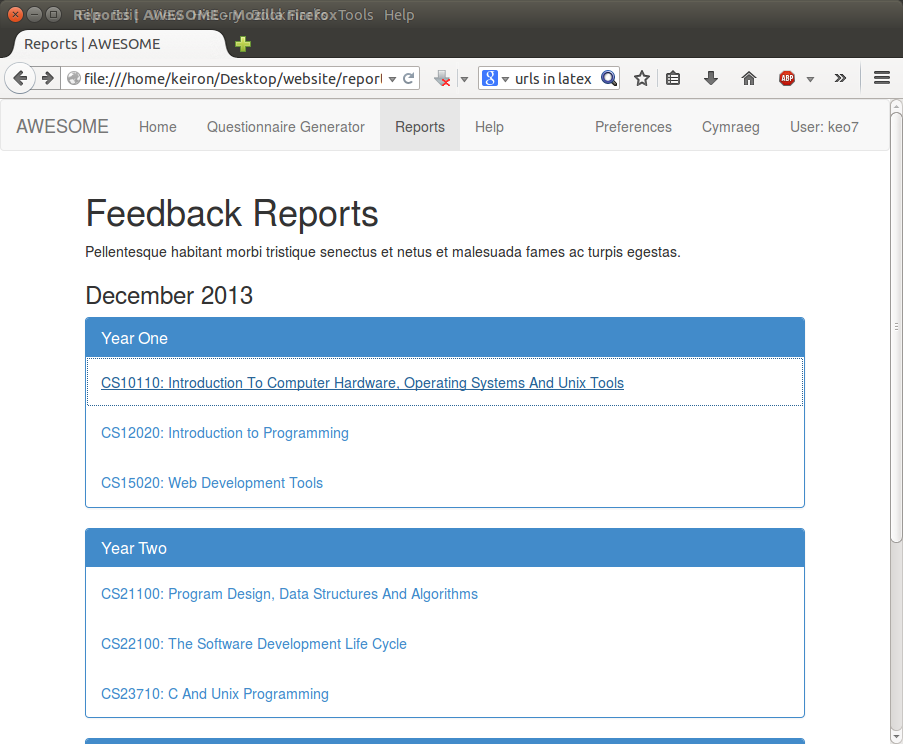
\includegraphics[width=0.85\linewidth]{images/uidesign/reportshome.png}
\end{figure}

\clearpage

\subsubsection{Report of a Module}

Once a user has selected a module/department to analyse they will be greeted by an in-depth report of how that module has done in previous surveys. It will consist of response figures outlining how many questionnaires were sent out and how many the department received.

Below that carefully formatted results of each question will be provided with HTML5 driven charts driven by Google Charts. If the user wants to analyse the results more closely then they can by seeing the direct results. Each chart/result will also contain a brief textual explanation.

\begin{figure}[h]
\centering
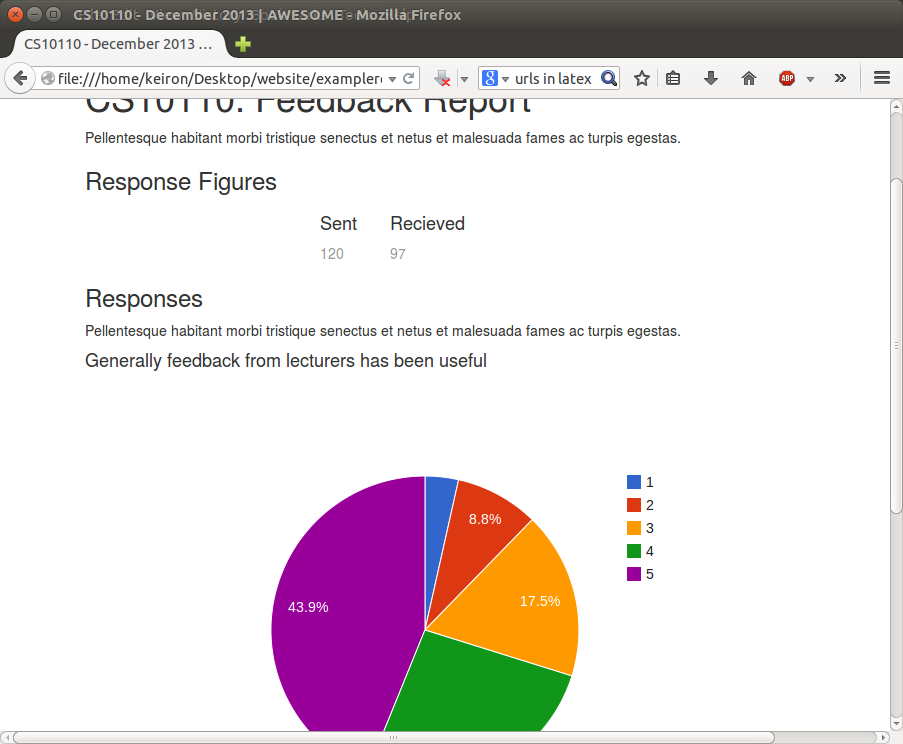
\includegraphics[width=0.85\linewidth]{images/uidesign/modulereport.png}
\end{figure}

\clearpage

\subsubsection{Help}

This page will mainly be text-based, but it may be a good idea to include video walking users through some of the more common issues they may encounter.

Not that there will be, my software is flawless. \footnote{I wish}

\begin{figure}[h]
\centering
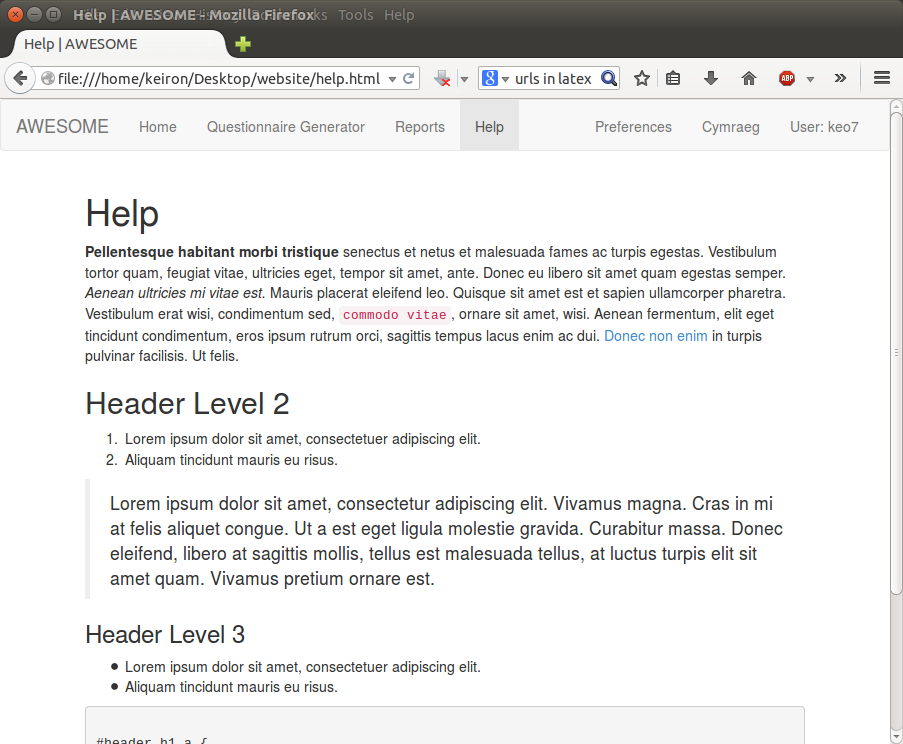
\includegraphics[width=0.85\linewidth]{images/uidesign/help.png}
\end{figure}

\clearpage
\section{Project Management}

\subsection{Gantt Chart}

The below figure is a Gantt chart, a visual representation of the project schedule. It describes the project milestones and task dependencies.

\subsection{Risk Analysis}

\clearpage

\section*{Document History}

\begin{center}
\begin{tabular}{|c | c | c | c | c |}
\hline
\textbf{Version} \cellcolor{gray!25} & \textbf{Date} \cellcolor{gray!25}& \cellcolor{gray!25}\textbf{Changes made to Document} &\textbf{ Changed by} \cellcolor{gray!25}\\
\hline
0.5 & 19-06-2014 & Completed UI & KeironO \\
\hline
0.2 & 17-06-2014 & Completed overview & KeironO \\
\hline
0.1 & 16-06-2014 & Initial creation & KeironO \\
\hline

\hline
\end{tabular}
\end{center}
\clearpage


\end{document}
